% Chapter Template

\chapter{Fundamentals on Synchrotron Radiation} % Main chapter title

\label{sr} % Change X to a consecutive number; for referencing this chapter elsewhere, use \ref{ChapterX}

\lhead{Chapter 2. \emph{Fundamentals on Synchotron Radiation}} % Change X to a consecutive number; this is for the header on each page - perhaps a shortened title

We call synchrotron radiation to the energy emitted by a charge which has a radial acceleration. It is produced in circular accelerators such as the LHC.
%----------------------------------------------------------------------------------------
%	SECTION 1
%----------------------------------------------------------------------------------------

\section{Radiation}
\begin{figure}
	\centering
  \begin{minipage}{\textwidth}
  	\centering
   	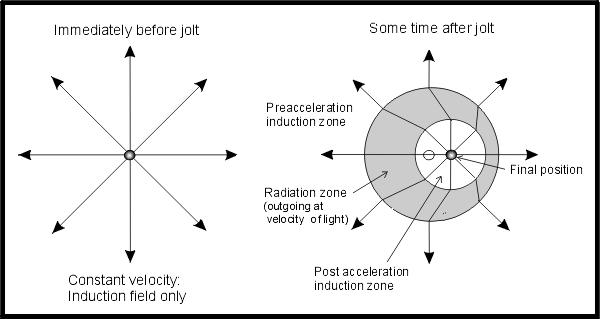
\includegraphics[width=3.5in]{Pictures/efields.jpg}
  		\caption{\label{fig:campos}
   			Electromagnetic field of a charge a) static b)after a short jolt }
   			\footnotesize{Picture taken from on \citep{img1}}
   \end{minipage}
\end{figure}
The idea of electromagnetic waves has always fascinated the mind of physicists around the world. In 1887 G. Hertz generated, emitted and received electromagnetic waves. This was an experimental proof of Maxwell's equations. The source of that radiation were oscillating charges.

First of all we should know that electromagnetic radiation is a consecuence of the finite velocity of light\citep{libro}. While a particle is at rest, or in a constant motion, it emits electric field lines radially out to infinity. If we suddenly accelerate this charge, the information of that acceleration travels with the speed of light, so that information is only known to the vicinity defined by: \begin{equation}
\Delta d \leq c* \Delta t  
\end{equation}
The distortion of these lines, which is traveling away from the charge is what we call electromagnetic radiation. This concept is shown in Figure \ref{fig:campos}.

\subsection{Conservation Laws}
The emission of electromagnetic radiation from free electrons is a classical phenomenon. We may therefore use a visual approach to gain some insight into conditions and mechanisms of radiation emission.
The emission of electromagnetic radiation involves two components, the electron and the radiation field. For the combined system energy–momentum conservation must be fulfilled. These conservation laws impose very specific selection rules on the kind of emission processes possible.
%-----------------------------------
%	SUBSECTION 2
%-----------------------------------
\section{Synchrotron Radiation}
The interest in electromagnetic theory grew in the mid 1940s with the development of the free electron radiation theories, mainly  because of the development of circular high energy electron accelerators. In 1944 Pomeranchouk showed that there was a limit to the betatron principle, and that there was also an energy limit due to the losses from electromagnetic radiation. The energy that charged particles lose to SR posed technological and economic problems to increase circular accelerators maximum energy. To surpass this limitation, circular accelerators started growing diametrically\citep{libro}.

When a relativistic beam of charged particles changes direction, it emits electromagnetic radiation, that can be seen as a search light, because it is highly collimated in the forward direction although it is broadband radiation, this is shown in Figure \ref{fig:synsim}. The shortness of this pulse is what indicates the observer it has detected synchrotron radiation with a broadband spectrum which is characterized by the critical photon energy. This energy depends solely on the paticle's energy and its bending radius as shown in equation \ref{eq:critical energy}, where $\varepsilon_{c}$ is the critical photon energy, $\omega_{c}$ is the critical photon frequency, $E$ is the particle's energy, and $\rho$ is the bending radius\citep{libro}. 
\begin{equation}
\label{eq:critical energy}
\varepsilon_{c} = \hbar\omega_{c} = \dfrac{3\hbar c}{2(mc^{2})^{3}}\dfrac{E^{3}}{\rho}
\end{equation}

There are particular characteristics of synchrotron radiation that depend on the magnetic devices used to generate that radiation, such as wigglers, undulators, wavelength shifters, etc. Nevertheless in this work we are only interested in bending magnets, furthermore superbends.

\begin{figure}
	\centering
  \begin{minipage}{\textwidth}
  	\centering
   	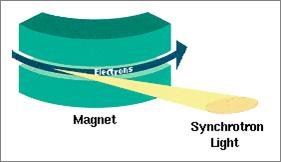
\includegraphics[width=3.5in]{Pictures/Syncrotron.jpg}
  		\caption{\label{fig:synsim}
   			Synchrotron radiation produced by a bending magnet.}
   			\footnotesize{Picture taken from \citep{fig:wiki1}}
   \end{minipage}
\end{figure}

\subsection{Superbends}
When a charged particle enters a magnetic field region, the particle is  deflected from its original trajectory perpendicularly to the magnetic field. The radius of this deflection depens only on the energy of the particle, its charge and the strength of the field. So we can express the critical photon energy as a function of the particle energy and the magnetic field. The numerical expression for an electron is shown in equation \ref{eq:51}\citep{libro}. 

\begin{equation}
\label{eq:51}
\varepsilon_{c}(keV) = 2.2183\dfrac{E^{3}(GeV^{3})}{\rho(m)}=0.66503E^{2}(GeV)B(T) 
\end{equation}

Where $B$ is the strength of the field. Sometimes the critical energy required for a given experiment is too high to be reached using regular magnets, or if we have a fixed $\rho$ and try to achieve maximum particle energy, as is the case of the LHC which had to fit in the LEP tunnel as mentioned in chapter \ref{ch:LHC}. In those cases regular magnets are replaced with much stronger and shorter superconducting electromagnets. Conventional bending magnet fields rarely exceed 1.5 T, but superconducting magnets can be operated at 5 to 6 T or higher\citep{libro}


%-----------------------------------
%	SUBSECTION 2
%-----------------------------------

\section{Radiation Power}
To know the total radiated power we integrate the Poynting vector $\vec{S}$ over a closed surface that keeps the charge inside. 
\begin{equation}
\label{eq:24}
P=\oint \vec{S}\cdot d\vec{A} 
\end{equation}
Doing this we find that the power radiating from a charged particle moving perpendicularly to a magnetic field is proportional to the fourth power of the particle's momentum and inversely proportional to the square of the bending radius\citep{libro}. For that reason, a slight increase in energy for a high energy particle leads to a huge increase of power loss due to synchrotron radiation. This is the reason why highest energy particle accelerators require a very large diameter.


%----------------------------------------------------------------------------------------
%	SECTION 2
%----------------------------------------------------------------------------------------


